\chapter{Resultate und Diskussion}
\label{chap:resultateDiskussion}
% =================================================================
\thispagestyle{fancy}
% =================================================================
Durchlaufend durch diese Arbeit wurden jeweils mittels QTI-Plots die Dicke/Lochdurchmesser mit deren Fehlern gefittet (Siehe Kapitel \ref{chap:auswertung} \textit{\nameref{chap:auswertung}}). Im Anhang unter \textit{\nameref{sec:messresultate}} sind die Werte der benutzten Objekten hinterlegt, mit welchen die gefitteten nun graphisch verglichen werden. Die Werte für die Strichgitter sind hier nicht nochmals aufgeführt, da für jene keine Fehlerrechnung gemacht wurde.\\
\begin{figure}[h]
\centering
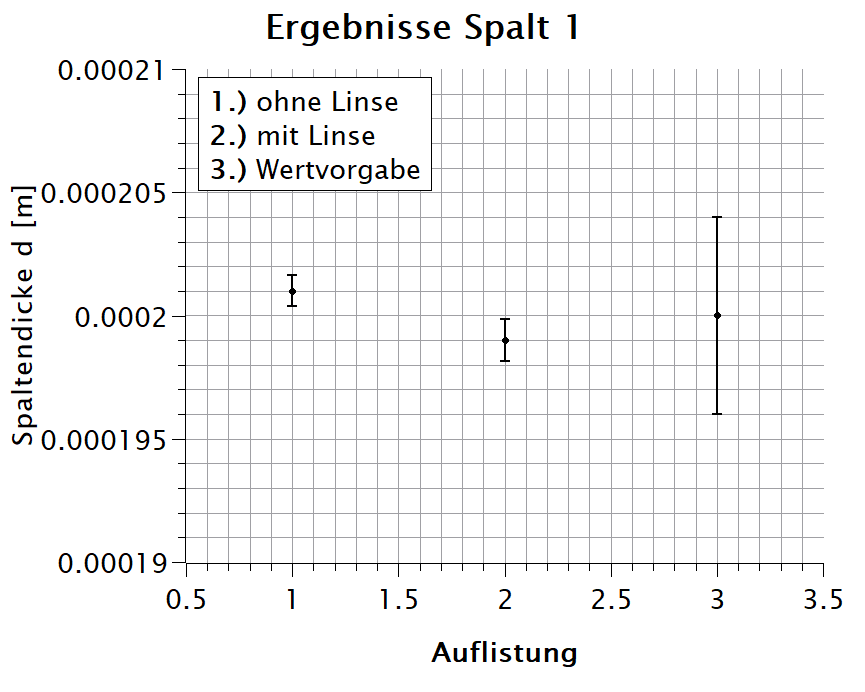
\includegraphics[width=\textwidth]{Bilder/ergebnisse_spalt1.png} 
\caption[Ergebnisse Spalt 1]{Deutlich zu sehen ist, dass die zwei Messreihen (mit und ohne Linse) im Bereich der Wertvorgabe liegen. Der numerische Wert der Wertvorgabe ist in der Abbildung \ref{fig:messresultate1} einzusehen. Somit ist die Spaltendicke verifiziert.}
\label{fig:ergSpalt1}
\end{figure}
\newpage
\begin{figure}
\centering
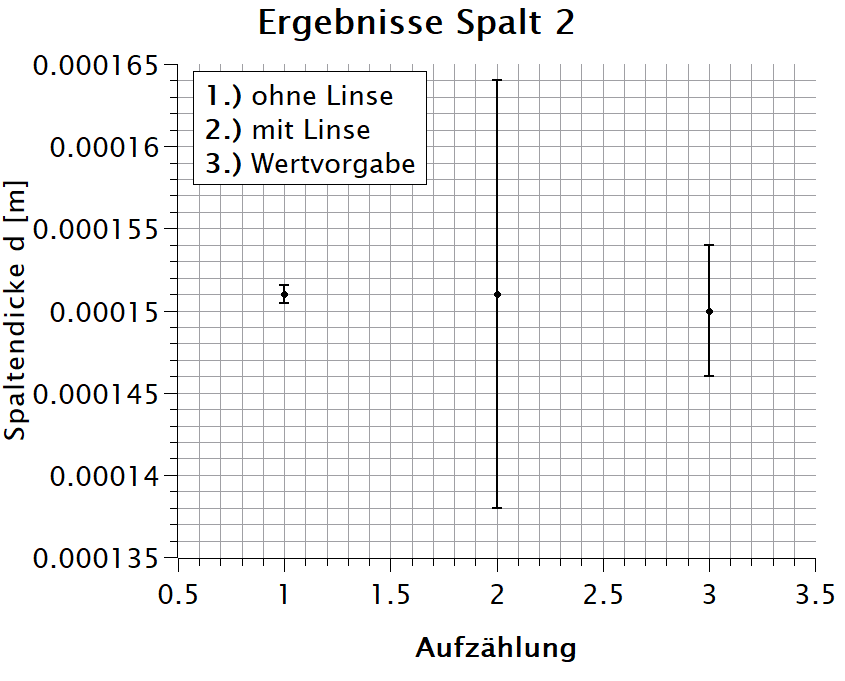
\includegraphics[width=\textwidth]{Bilder/ergebnisse_spalt2.png} 
\caption[Ergebnisse Spalt 2]{Auch hier liegen beide gemessenen Werte innerhalb des Bereiches, welcher von der Wertvorgabe für die Spaltendicke vorgegeben ist. Allerdings ist die Unsicherheit mit der Linse etwas höher, was durch ungenaues Ablesen kausieren könnte. Dennoch ist die Spaltendicke verifiziert.}
\label{fig:ergSpalt2}
\end{figure}
\newpage
\begin{figure}
\centering
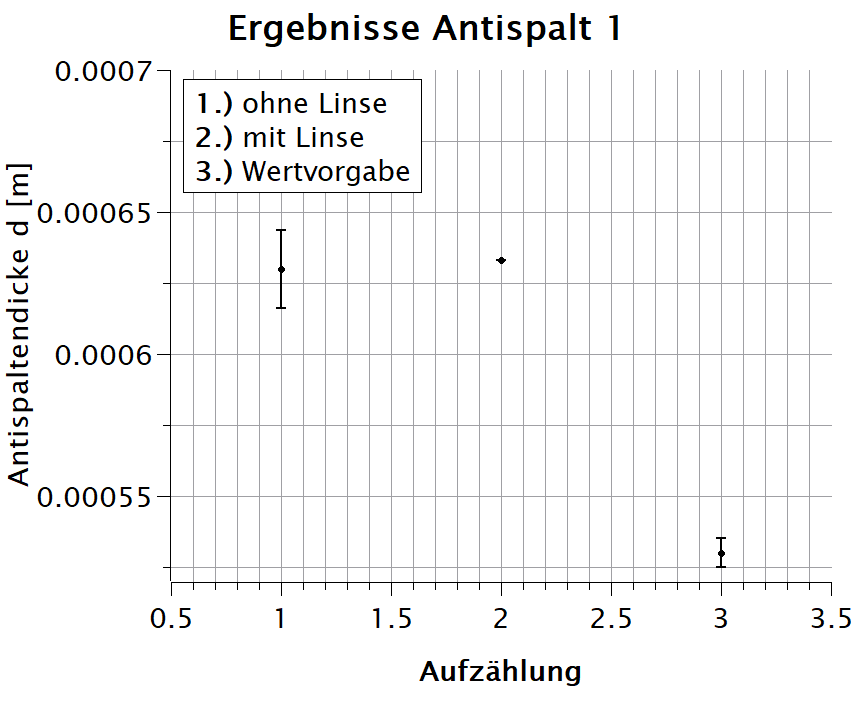
\includegraphics[width=\textwidth]{Bilder/ergebnisse_antispalt1.png} 
\caption[Ergebnisse Antispalt 1]{Hier weicht das Gemessene um ca. 100$\mu$m vom vorgegebenen Wert ab. Dies könnte durch falsches Aufschreiben des Antispalts passiert sein. Denn beide Messreihen liegen sehr nahe beieinander. Zudem sind im Allgemeinen die Messwerte beim Antispalt etwas ungenauer. Es könnte auch auf die falsche Weise gemessen worden sein.}
\label{fig:ergAntispalt1}
\end{figure}
\newpage
\begin{figure}
\centering
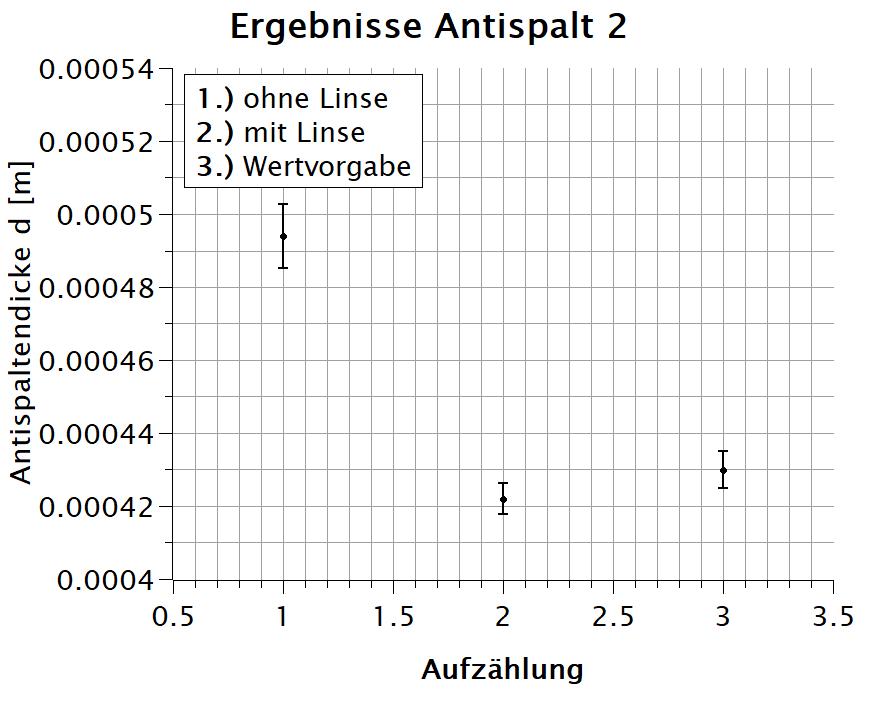
\includegraphics[width=\textwidth]{Bilder/ergebnisse_antispalt2.png} 
\caption[Ergebnisse Antispalt 2]{Die gemessenen Werte liegen ziemlich nahe an der Wertvorgabe beim 2. Antispalt. Besonders die Messreihe mit Linse liegt nur leicht ausserhalb des vorgegebenen Wertes. Auch hier, wie bei Abbildung \ref{fig:ergAntispalt1} könnten die Messwerte genauer sein, wenn die Maximas, anstatt die Minimas gemessen worden wären.}
\label{fig:ergAntispalt2}
\end{figure}
\newpage
\begin{figure}
\centering
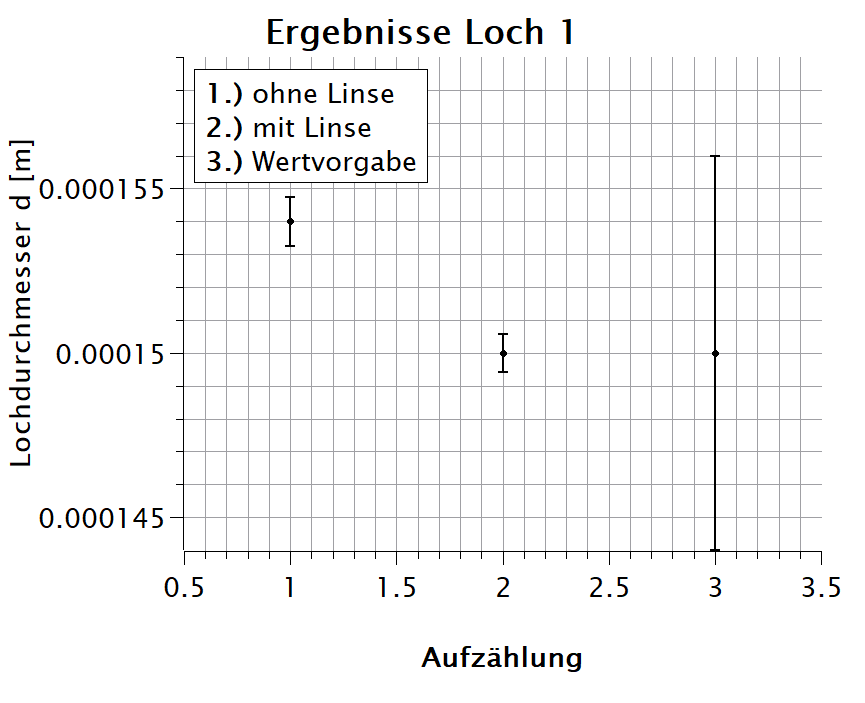
\includegraphics[width=\textwidth]{Bilder/ergebnisse_loch1.png} 
\caption[Ergebnisse Loch 1]{Diese Messreihen mit dem Objekt \textit{Loch} liegen ziemlich genau im vorgegebenem Bereich. Der Lochdurchmesser kann somit als verifiziert betrachtet werden.}
\label{fig:ergLoch1}
\end{figure}
\newpage
\begin{figure}
\centering
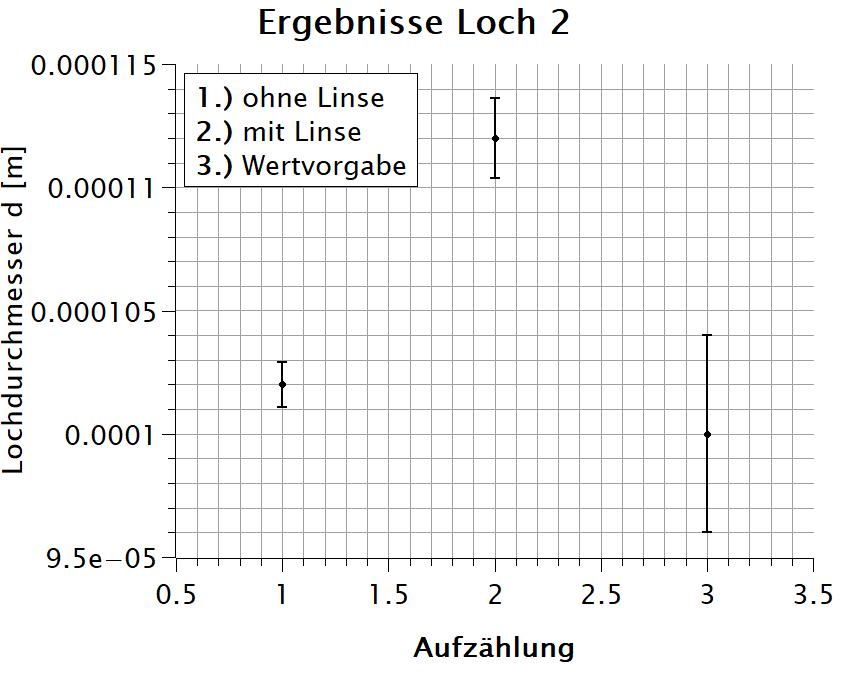
\includegraphics[width=\textwidth]{Bilder/ergebnisse_loch2.png} 
\caption[Ergebnisse Loch 2]{Hier sind die beiden Messreihen etwas zerstreuter als bei der Abbildung \ref{fig:ergLoch1}. Die Messreihe ohne Linse liegt hier deutlich besser im vorgegebenen Bereich als der ohne Linse. Allerdings beträgt die Abweichung nur 6$\mu$m.}
\label{fig:ergLoch2}
\end{figure}
\newpage